
\chapter{Algorithm Validation}\label{ch:validation} 

To verify the performance of the algorithm as discussed in Chapter \ref{ch:algorithm} this chapter explains how by  experiment the algorithm output is compared with microscopic profilometry data. First the experimental process is explained. Then height and width measurement from microscopic data is discussed and at last calibration between data from the microscopic and the algorithm is presented with validation of the algorithm.

\section{Validation Process}

% Explain briefly all aspects taken in the Validation Process.
% More detailed discussions on Profilometry Measurement and Algorithm, Calibration and Validation.
% Reason is that Line Scanning and Detection algorithm are already discussed.
To validate the detection algorithm from Chapter \ref{ch:algorithm} an experiment is conducted where two types of measurement are performed. The first measurement is performed by a microscope and the second by the detection algorithm. Since the microsope in comparison is much more accurate it is used to validate the measurement from the detection algorithm. Figure \ref{fig: process} shows an overview of the validation process.  
\begin{figure}[ht]
\centering
\begin{tikzpicture}[node distance = 2.5cm, auto]
    % Place nodes
    \node at (1,0)[block] (middle_0) {Material Printing};
    \node at (0,1)[block_scan, below of=middle_0, left of=middle_0] (left_1) {Line Scanning};
    \node at (2,2)[block_prof, below of=middle_0, right of=middle_0] (right_1) {Profilometry Measurement};
    \node at (1,3)[block_scan, below of=left_1] (left_2) {Scanning Algorithm};
    \node at (2,4)[block_prof, below of=right_1] (right_2) {Profilometry Algorithm};
    \node at (1,5)[block, below of=right_2, right of=left_2] (middle_3) {Calibration};
    \node at (1,6)[block, below of=middle_3] (middle_4) {Validation};
	\node[text centered, text width = 2cm] at (1,-1.5) {Deposition \\ Line};
	\node[text centered, text width = 2cm] at (1,-6) {Height \& \\ Width};
    % Draw edges
    \path [line] (middle_0) -- (left_1);
    \path [line] (middle_0) -- (right_1);
    \path [line] (left_1) -- node {Images} (left_2);
    \path [line] (right_1) -- node {Height Map}(right_2);   
    \path [line] (left_2) -- (middle_3);
    \path [line] (right_2) -- (middle_3);   
    \path [line] (middle_3) -- node {Calibration Model} (middle_4);          
\end{tikzpicture}
\caption{Experimental Validation Process}
\label{fig: process}
\end{figure}
The process starts with the printing of a deposition line. The top of Figure \ref{fig: setup} shows the setup used for printing. The container holding the silicone is pressurized and material is depositied onto the bed through the nozzle. This silicone is then cured by the UV lamp. 
\begin{figure}[ht]
\centering
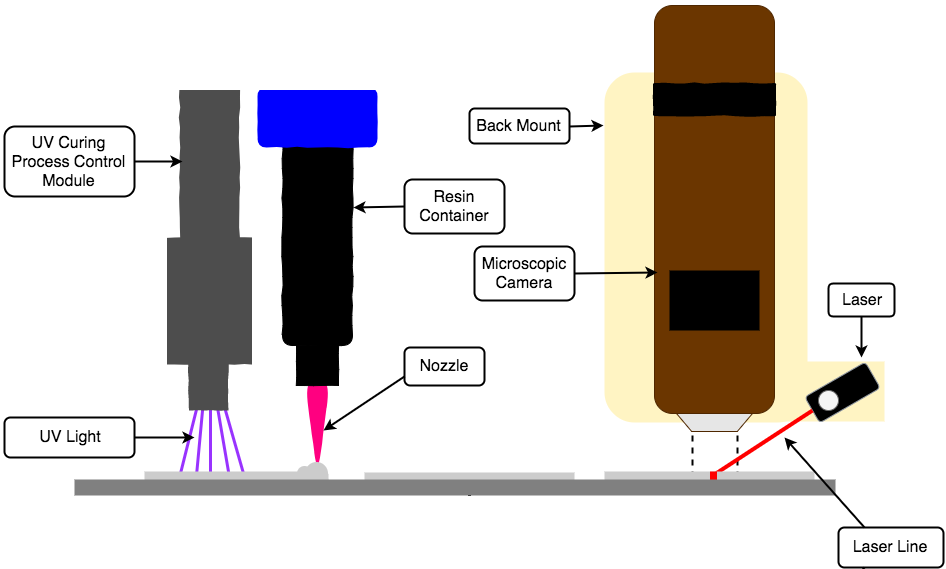
\includegraphics[width=1\linewidth]{VisionSetup} 
\caption{Experimental setup.}
\label{fig: setup}
\end{figure}
The deposited line is then scanned using the measurement setup as discussed in Chapter \ref{ch:hardware} and measured using the microscopic profilometry system as shown in Figure \ref{fig: keyence}. The camera from the line scanner produces RGB images which are reduced to a height and width in pixels by the detection algorithm. The micrscope produces a height map which is reduced by the profilometry algorithm to a height and width in physical units. The height and width measurements of the detection algorithm are then calibrated against the profilometry results and the error of the calibration model is discussed at the validation step. 
\begin{figure}[ht]
\begin{subfigure}{0.25\textwidth}
\centering
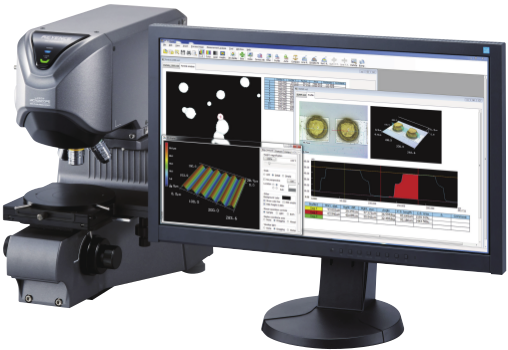
\includegraphics[width=1\linewidth]{microscope} 
\caption{Keyence VK-X250K}
\label{fig: keyence}
\end{subfigure}
\begin{subfigure}{0.75\textwidth}
\centering
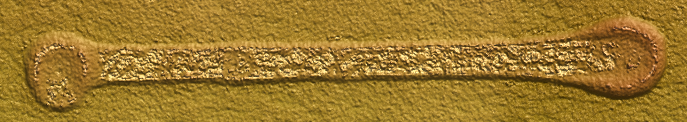
\includegraphics[width=1\linewidth]{micro_out}
\caption{Typical Silicon Line Profilometry Measurement}
\label{fig:profile2}
\end{subfigure}
\caption{Microscopic Profilometry}
\label{fig:}
\end{figure}

\section{Profilometry Measurement and Algorithm}

A typical measurement performed by the microscope is shown in Figure \ref{fig:profile}. This visualization is a large 2D array consisting of large integer values. 

% Make 3D plot
\begin{figure}[ht]
\centering
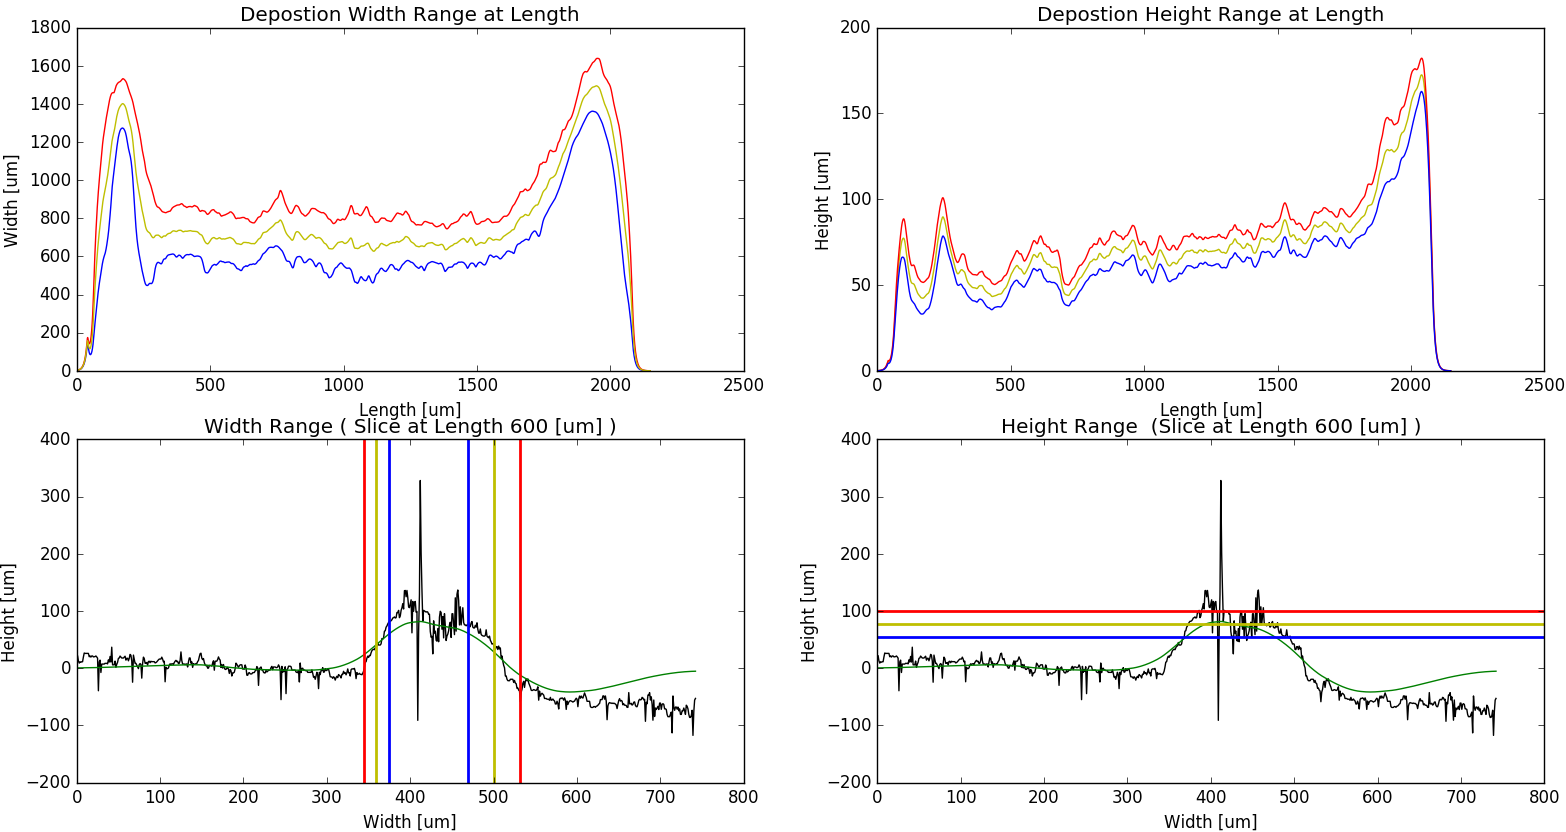
\includegraphics[width=1\linewidth]{micro} 
\caption{Experimental setup.}
\label{fig: setup}
\end{figure}

\blindtext[2]

\section{Calibration}

Sampling-Time Scaling

autocorrelation to find best fit.


Talk about the fact that first all lines are deposited. Afterwards teh measurement takes place at constant speed. Therefore having a constant sampling time and therefore equal space between measurements. Since the sampling time is unkonwn the output is scaled in time to match 
Talk about the experiment. 

\section{Validation}
% Talk about the need for validation and calibration
Talk about how the algorithm is validated against data for microscopy. also talk about that is calibrated that way to related pixels to physical measures.

% Talk about the microscope used for these purposes.
\blindtext[1]



% Talk about the data it generates with it noise and outliers.
% Also talk about low pass filtering to overcome that. 
% Furthermore talk about using the triangle method to determine width.
% ATTENTION height should still be decided upon.
\blindtext[1]



\blindtext[1]



\blindtext[1]